\documentclass[10pt]{article}

% Lines beginning with the percent sign are comments
% This file has been commented to help you understand more about LaTeX

% DO NOT EDIT THE LINES BETWEEN THE TWO LONG HORIZONTAL LINES

%---------------------------------------------------------------------------------------------------------

% Packages add extra functionality.
\usepackage{times,graphicx,epstopdf,fancyhdr,amsfonts,amsthm,amsmath,algorithm,algorithmic,xspace,hyperref}
\usepackage[left=1in,top=1in,right=1in,bottom=1in]{geometry}
\usepackage{sect sty}	%For centering section headings
\usepackage{enumerate}	%Allows more labeling options for enumerate environments 
\usepackage{epsfig}
\usepackage[space]{grffile}
\usepackage{booktabs}
\usepackage{forest}

% This will set LaTeX to look for figures in the same directory as the .tex file
\graphicspath{.} % The dot means current directory.

\pagestyle{fancy}

\lhead{Final Project}
\rhead{\today}
\lfoot{CSCI 334: Principles of Programming Languages}
\cfoot{\thepage}
\rfoot{Fall 2023}

% Some commands for changing header and footer format
\renewcommand{\headrulewidth}{0.4pt}
\renewcommand{\headwidth}{\textwidth}
\renewcommand{\footrulewidth}{0.4pt}

% These let you use common environments
\newtheorem{claim}{Claim}
\newtheorem{definition}{Definition}
\newtheorem{theorem}{Theorem}
\newtheorem{lemma}{Lemma}
\newtheorem{observation}{Observation}
\newtheorem{question}{Question}

\setlength{\parindent}{0cm}


%---------------------------------------------------------------------------------------------------------

% DON'T CHANGE ANYTHING ABOVE HERE

% Edit below as instructed

\begin{document}
  
\section*{Lab 9 - Squares And More (SAM)}

% Full name: Squares And More: Useless Evaluated Language

Gerardo Morales, Will Confoy

\subsection{Introduction}

Art is hard. How hard varies from person to person but for those who are not artistically inclined, it can be really difficult to get over the initial hurdle of making what's in your head appear on canvas. Squares And More (SAM) helps to remove this barrier, by providing a rigorous language for creating regular polygons of nearly any configuration. Additionally, SAM supports a syntax that is easy to understand for anyone fluent in English, further increasing its usefulness.

\vspace{.1cm}

SAM's usage especially lessens the burden on anyone who is disabled or has difficulty with fine motor skills. So long as you can put words on a screen, you can use SAM to produce the exact image you want, so long as that image is made up of regular polygons. This coupled with the fairly natural language approach of SAM means that SAM works well with the many diverse methods by which people have found to interface with computers.

\subsection{Design Principles}

While designing SAM, we kept in mind two main principles: ease of use and abstraction. We wanted to ensure that SAM was easily understandable to English speakers so that it would be easy for people who hadn't seen it before to hop in and begin writing programs, and being able to put the image in their brain on canvas. Of course, there are some specifics that require user input, as it is a rigorous language. However, we did our best to abstract as much of the definitions away from the sight of the user, using the minimum definitions of shapes possible to deterministically define shapes. For example, you really only need a point, a distance, a number of sides, and an orientation to fully define any regular n-gon.

\subsection{Examples}

Here are a few sample programs:

\begin{verbatim}
    2 4-gon with radius 4 and center (1,1), step [1], color[0x6b0df0, 0xa73387], 
    centerDelta (0,-1), uniform (0,1) and granularity 2
\end{verbatim}

This will produce 2 concentric squares, one with radius 4 and one with radius 5. They will have the color corresponding to their index in the color array, and the second square will have a center moved down by 1 in the y direction. They will both have wavy lines, split into 3 segments with 2 points besides the endpoints, which are deviated from the original line by picking from the uniform(0,1) distribution.

and another:

\begin{verbatim}
    4 10-gon with radius 3 and center(1,1), step[1,2,1], 
    color[0xf9c406, 0xdc4dda, 0x995668, 0xf9c406, 0x2cf249], centerDelta(-5,0.2),
    laplace(0,10) and granularity 5
\end{verbatim}

This will produce 4 concentric 10-gons, with radii 3,4,6,7. They will have the color corresponding to their index in the color array, and each one will have their center moved -5 in the x direction and 0.2 in the y direction compared to the previous 10-gon. They will both have wavy lines, split into 6 segments with 5 points besides the endpoints, which are deviated from the original line by picking from the laplace(0,10) distribution.

and finally:

\begin{verbatim}
    1 7-gon with radius 20 and center(1,1), step [], color [0x5f28a8],
    centerDelta(1,1), normal(0,1) and granularity 0
\end{verbatim}

This will produce 1 7-gon with radius 20 and color 0x5f28a8. Step and centerDelta are irrelevant because there's only one polygon, and since granularity is 0, each of the edges will be totally straight.

\subsection{Language Concepts}

The core ideas can essentially be boiled down into what a regular n-gon is, and different attributes that they may have, such as orientation, size, and color. For some of the specific syntax, it might be useful to understand what an array is, as we use them to specify values for different polygons. Since we are only exposing creation of 1 type of shape, users don't need to worry about many different primitives or combined forms. Underneath the hood, there will be plenty of points, lines, and whatnot, but that's all abstracted away. For example, a polygon is a composed of a point, a radius, a color, and a rotation (in degrees). We ask the user for all of the data, but it's in English and we handle putting it all together.

\subsection{Syntax}
We will write our syntax in a sort of pseudo BNF form- we say pseudo because it contains ideas that we have not seen in BNF form before. In particular, it contains exponents, such as in $<expr>^2$, where it represents exactly 2 $<expr>$. It's not totally rigorous yet, but it serves to give the right idea. Additionally, the first $<n>$ in the $<ngon>$ is represented later on with $N$, because the number of consecutive terms we want in later parts depends on it.

\begin{align*}
    <expr> &:= <ngon>^+ \\
    <ngon> &:= <n>\text{\textvisiblespace}<n>-\text{gon\textvisiblespace with\textvisiblespace radius }<f> \text{ and\textvisiblespace center}(<f>,<f>),\\
    &\quad \text{ step } <step>, \text{ color} <color>, \text{ centerDelta} (<f>,<f>),\\
    &\quad <dist> \text{ and granularity } <n> <newline>^+\\
    <n> &:= <digit>^+ \\
    <neg n> &:= -<n>\\
    <int> &:= <n> | <neg n>\\
    <digit> &:= x \in \mathbb{Z}_{10} \\
    <f> &:= <int>.<n> \\
    <step> &:= \left[<steps>^{N-1}\right] \\
    <steps> &:= <int>,<int> \\
    &\quad\mid <int>\\
    <color> &:= [<hex>^N] \\
    <hex> &:= \#<hdigit>^6\\
    <hdigit> &:= 0\mid 1\mid 2\mid\ldots | F\\
    <dist> &:= <name>(<f>,<f>)\\
    <name> &:=\text{``normal'' }\mid \text{``uniform'' }\mid\text{``laplace'' }\mid\text{``fish''} \\
    <newline> &:= \text{`}\symbol{92}n\text{'}
\end{align*}


\subsection{Semantics}

\begin{enumerate}
    \item Primitive values:

        There are three main primitives- ints, floats, and hex values, as just about everything boils down to them eventually, beside the specific names for probability distributions. The ints and floats are how the user provides information to the program on the specifications for almost all of the attributes of their n-gon, including what n is, and the hex values are there to allow the user to give very specific colors for their n-gons.
        
    \item Actions or compositional elements:

        Through the syntax of the language, primitives are combined to form a series of n-gons. These n-gons are the form that users will be thinking in, rather than the primitives. Everything about an n-gon can be defined with some combination of the primitives, which is why they are a combined form. The way in which they combine the forms is based on the specific syntax, which is fairly strict to ensure it remains readable and easy to understand. Additionally, the primitives combine to form lists/arrays.

    \item What types will be used in your AST?

        Our types will be very similar to the BNF we have drawn out. Primitives will be stored as ints, floats, and strings. Ints and floats are for $<n>$ and $<f>$, but the hex values will be stored as strings because we only need to put them into the SVG file format. However, we'll be making algebraic data types for most of the types in our BNF up in the syntax section. The exceptions are the ones like $<n>$, where we needed to use $<digit>$ in our BNF, but int is convenient to use in F\# and works just as well.
        
    \item How do the abstract syntax trees fit together

        Here are the ASTs for the three example problems given above. The size of the second layer of the tree was so large that it was breaking the forests package, so we had to do it by hand and take a picture. Same for the evaluation in the last part of the question.
        \begin{figure}[h]
            \centering
            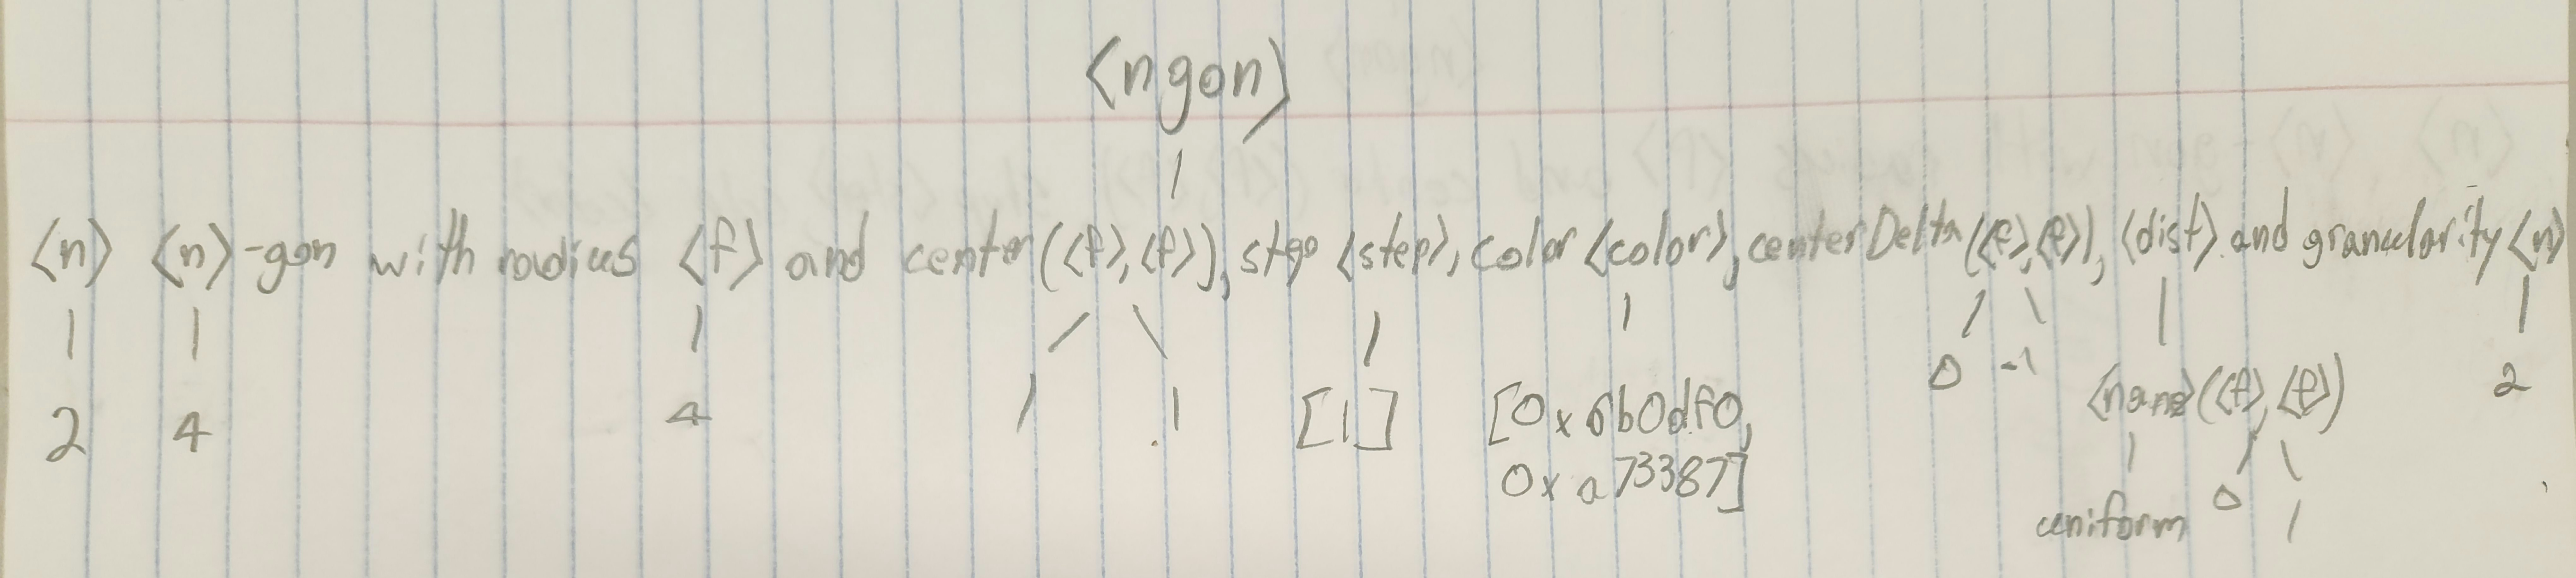
\includegraphics[scale=.05]{2,4.jpg}
        \end{figure}
        \begin{figure}[h]
            \centering
            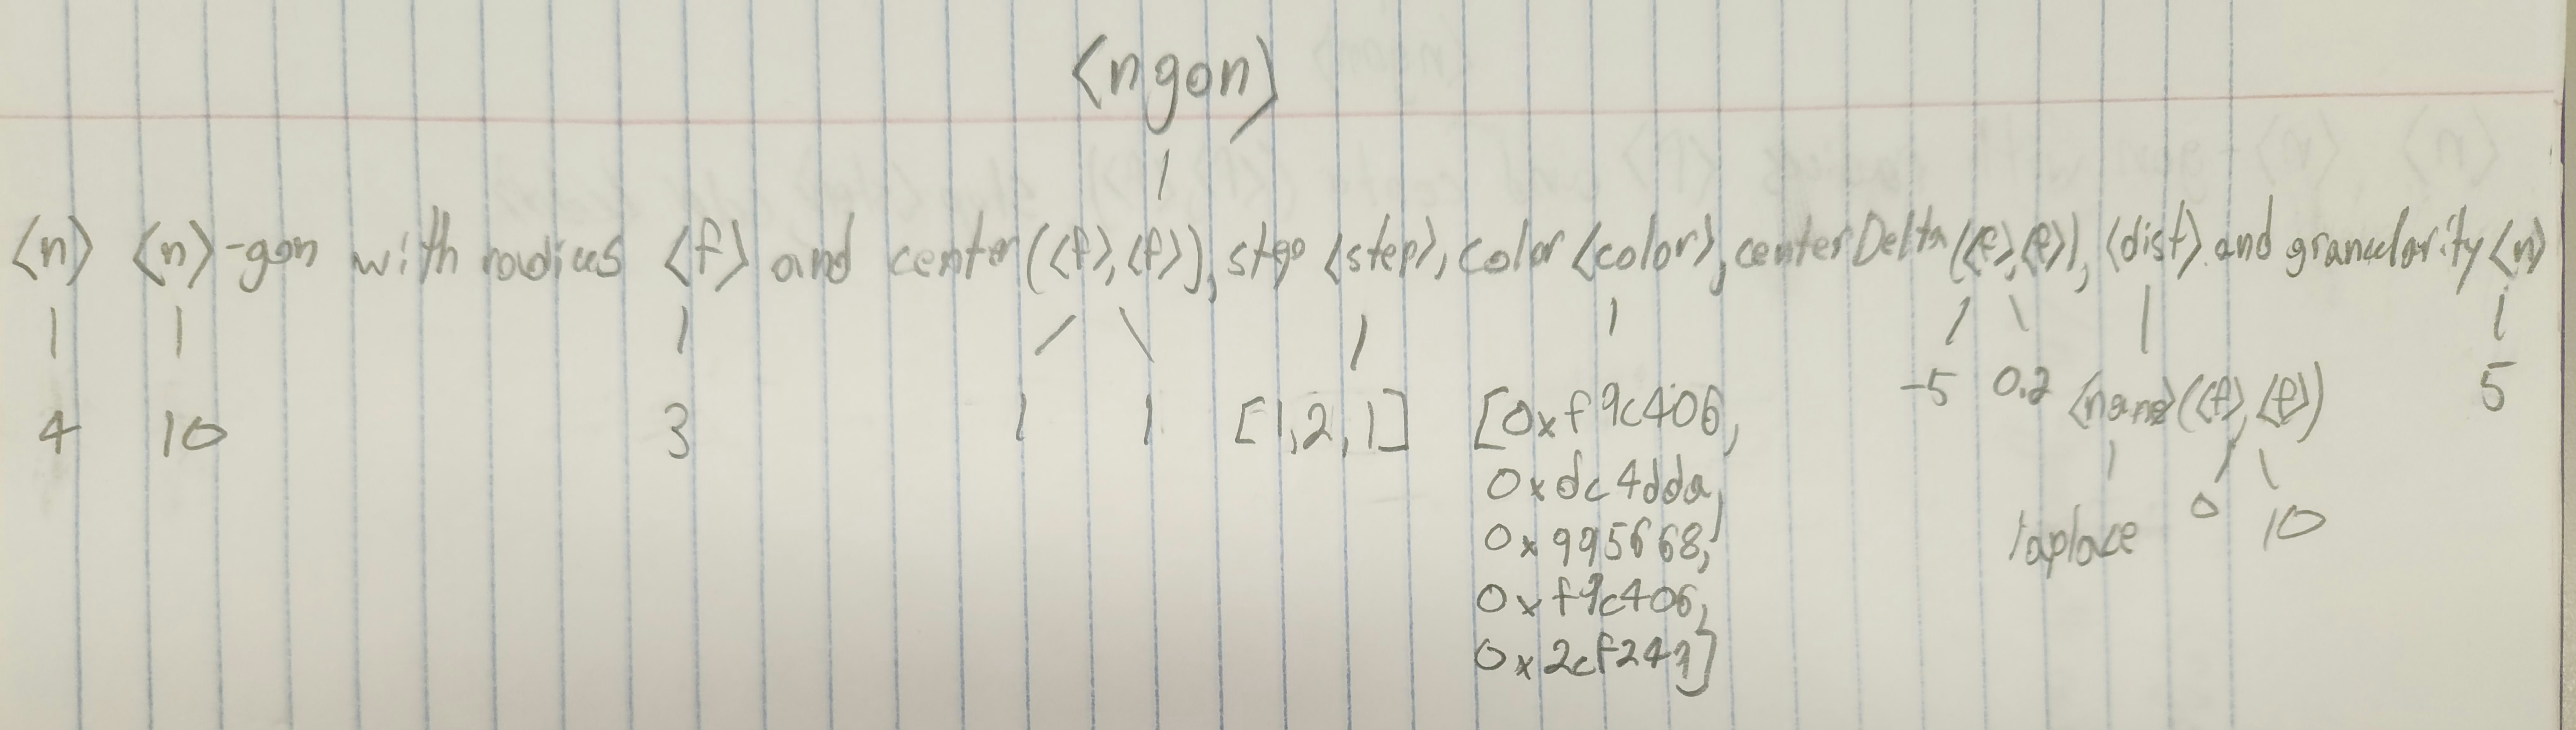
\includegraphics[scale=.05]{4,10.jpg}
        \end{figure}
        \begin{figure}[h]
            \centering
            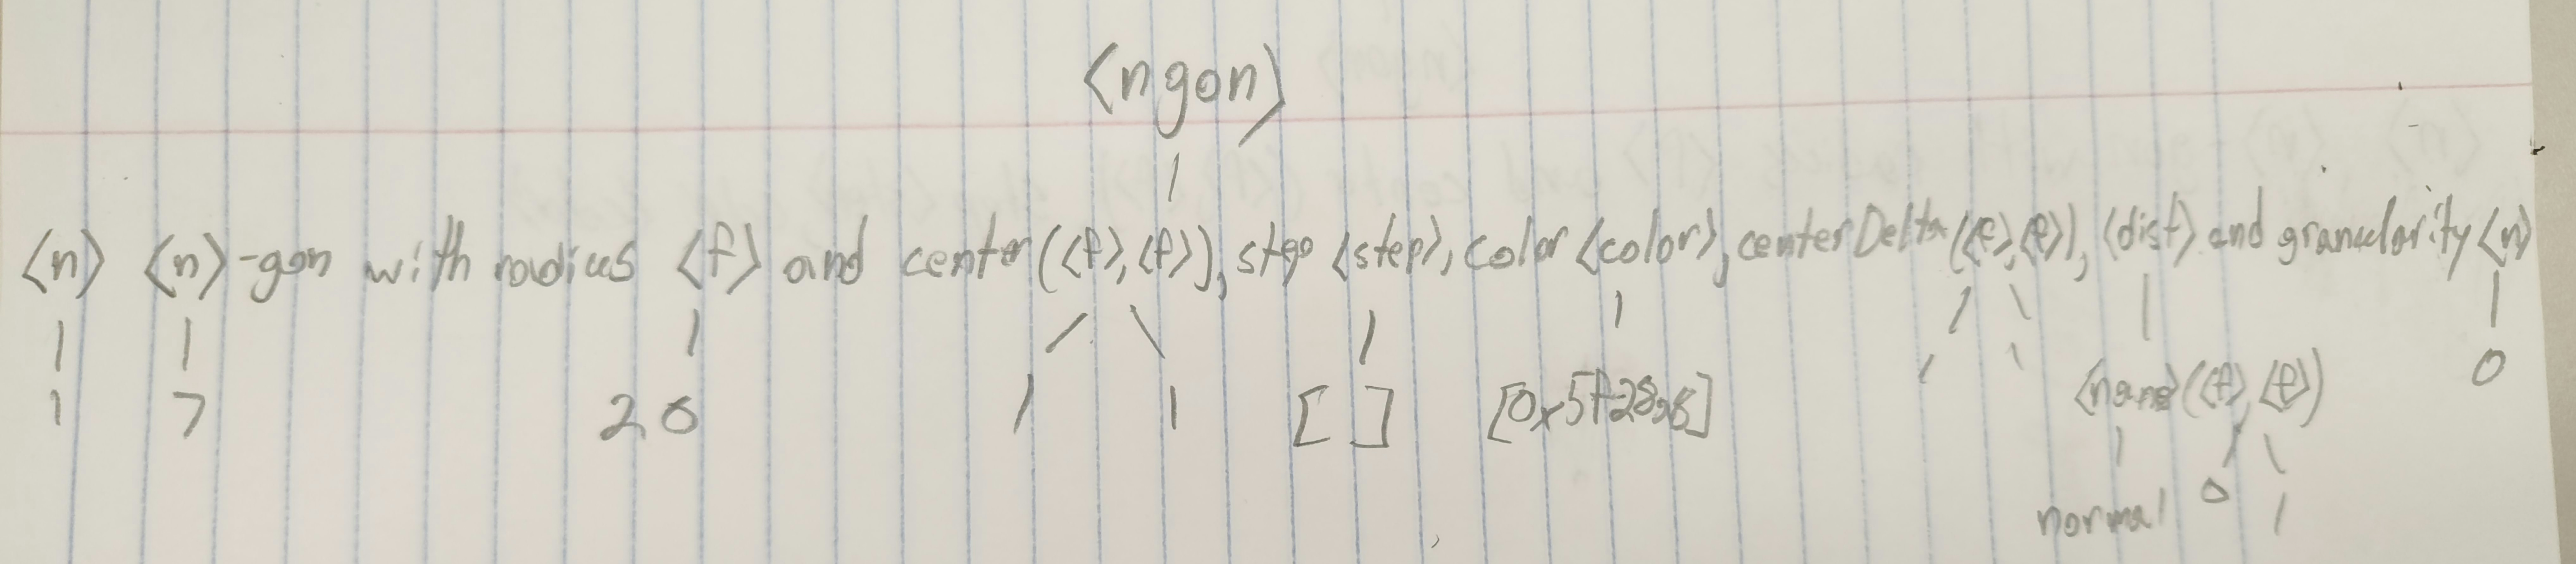
\includegraphics[scale=.05]{1,7.jpg}
        \end{figure}
        \newline
        \newline
        \newline
        \newline
    \item How is it evaluated (does it read any input, what is the output, demonstrate evaluation)

        The programming language doesn't need any input besides the program itself, which can either be typed out in the command line or put into a file and read from the file by F\#.

        As output, it will return the code for an SVG file that has the described image, much like we did with linelang in class. Similarly, it can be piped into a file to make the file contain the outputted program/image.

        For parsing the AST, we traverse it and as we do, we fill out the data for an n-gon object, which we then evaluate to produce the output that we want. Below is a picture of the AST for the third example in section 0.3.
        \begin{figure}[h]
            \centering
            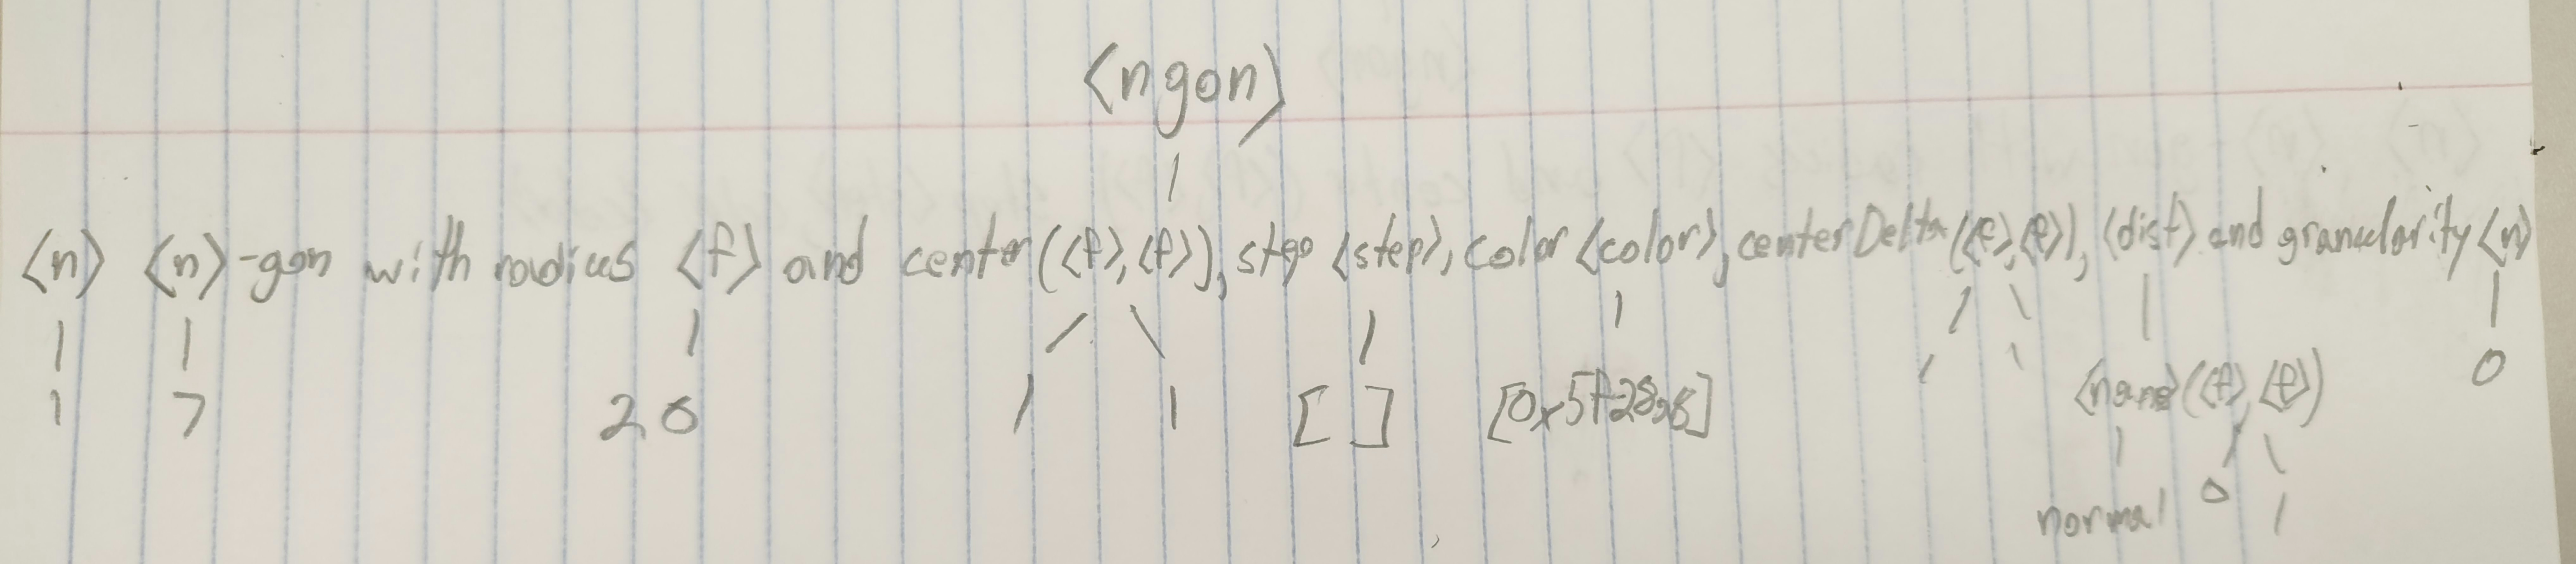
\includegraphics[scale=.05]{1,7.jpg}
        \end{figure}

        
        A post order traversal will construct an object akin to the one below. Note that the empty list for step would contain floats, but since $N=1, N-1=0$ so it must be empty.
        \begin{verbatim}
            ngon = {
                num = 1;
                numSides = 7;
                radius = 20;
                center = (1,1);
                step = [];
                color = ["#f9c406"];
                centerDelta = (1,1);
                dist = {name = "normal"; param = (0,1)};
                granularity = 0;
            }
        \end{verbatim}
        
\end{enumerate}

% DO NOT DELETE ANYTHING BELOW THIS LINE
\end{document}